\documentclass[border=10pt]{standalone}

\usepackage{tikz}
\usepackage{tikzsymbols}
\usetikzlibrary{calc,patterns,shapes.geometric}

\def\centerarc[#1](#2)(#3:#4:#5){\draw[#1] ($(#2)+({#5*cos(#3)},{#5*sin(#3)})$) arc (#3:#4:#5);}

\begin{document}
	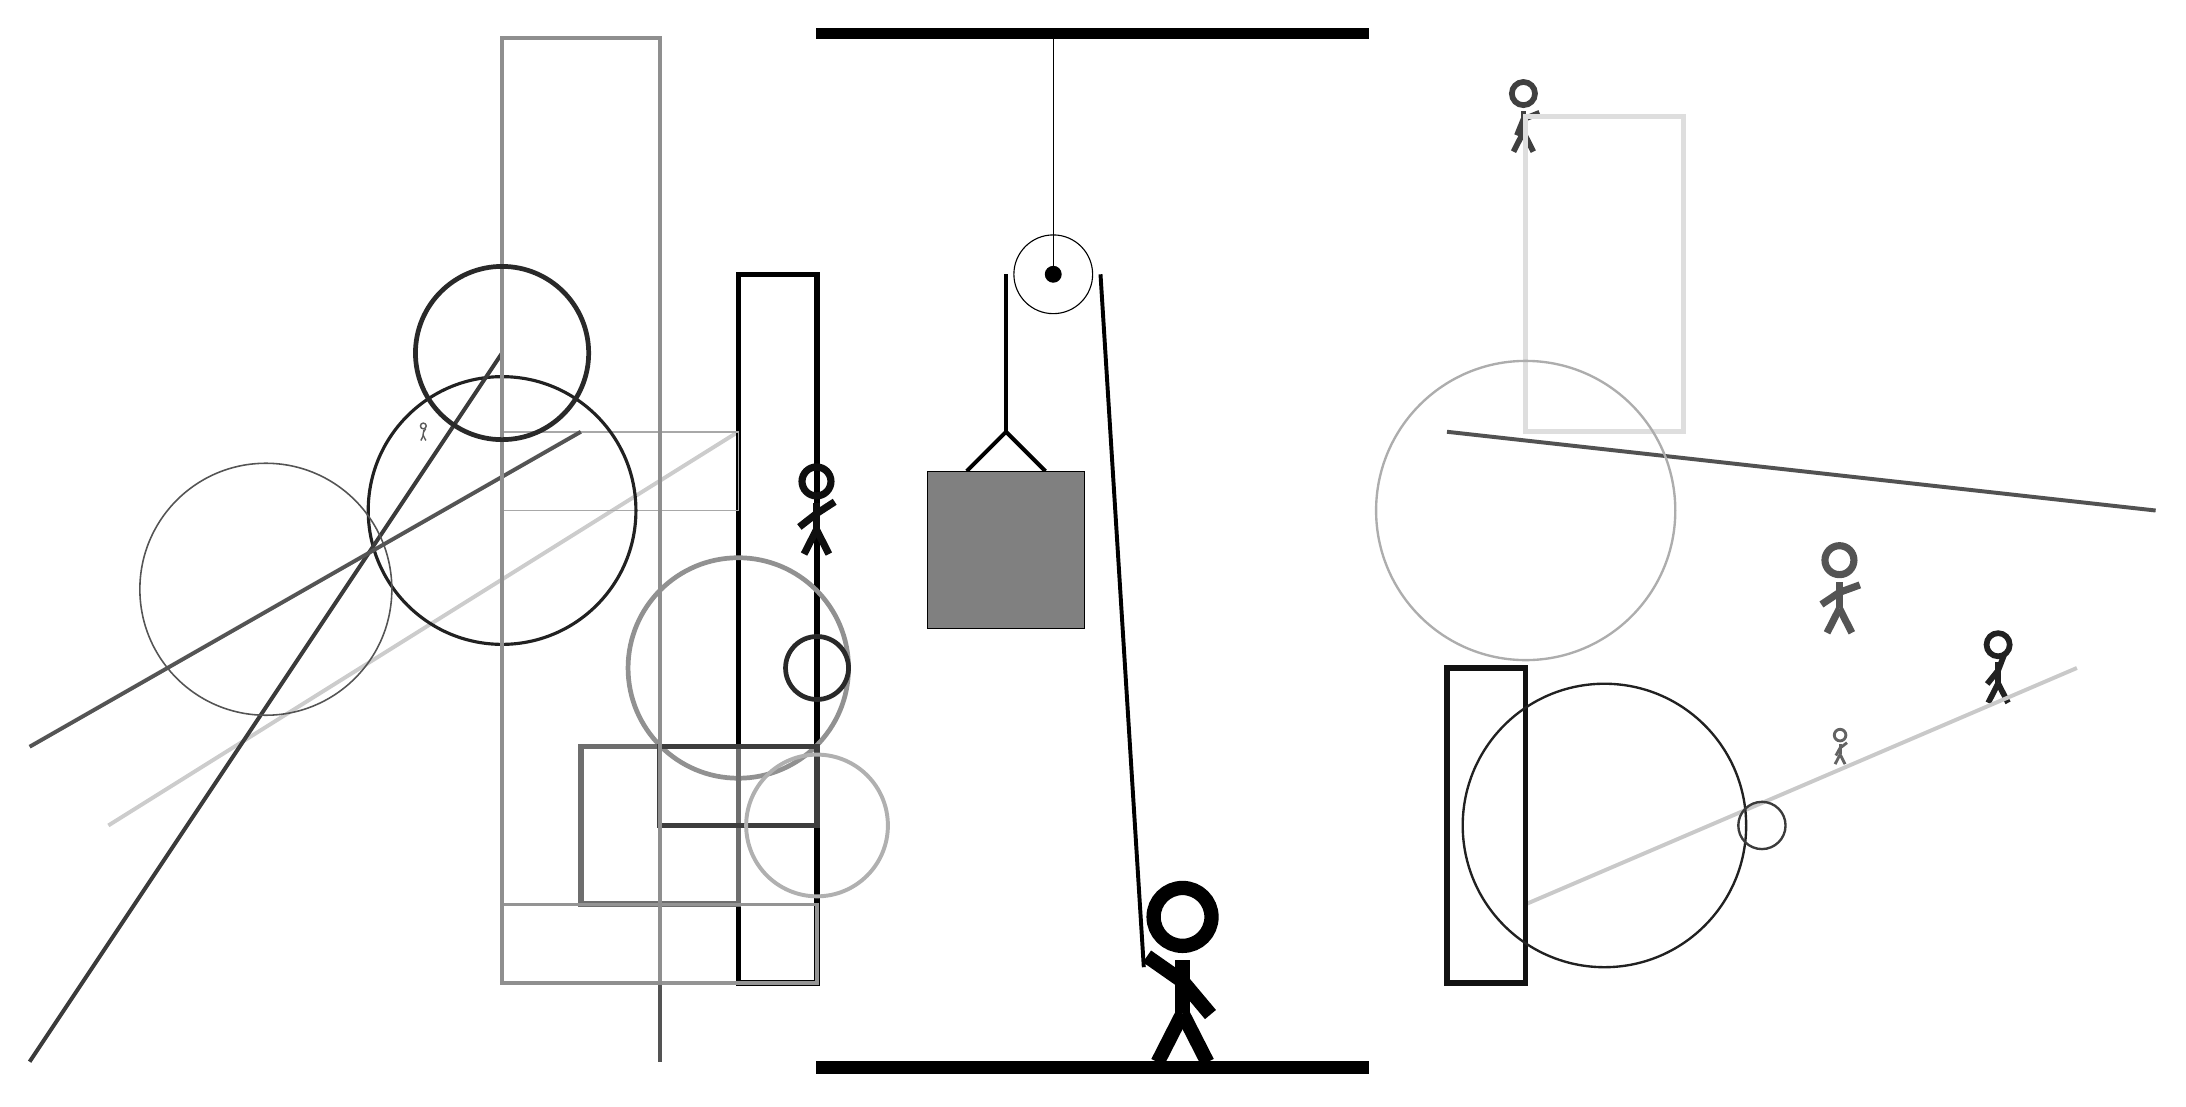
\begin{tikzpicture}
		%%%%% START %%%%%
		
		\draw[fill=black] (-2, 10) rectangle (5, 10.125);
		
		\draw (1, 7) circle (0.5);
		\draw[fill=black] (1, 7) circle (0.1);
		\draw (1, 10) -- (1, 7);
		
		\draw[line width=0.5mm] (-0.1, 4.5) -- (0.4, 5.0) -- (0.9, 4.5);
		\draw[fill=black!50] (-0.6, 4.5) rectangle (1.4, 2.5);
		
		\node[line width=0.6mm, color=black!75] at (7, 9) {\Strichmaxerl[4][68][22]};
		
		\draw[line width=0.5mm, color=black!20](-3, 5) -- (-11, 0);
		\node[line width=0.5mm, color=black!87] at (13, 2) {\Strichmaxerl[4][51][69]};
		\draw[line width=0.5mm, color=black!21](7, -1) -- (14, 2);
		
		\draw[line width=0.7mm, color=black!100] (-2, 7) rectangle (-3, -2);
		\draw[line width=0.2mm, color=black!34] (-3, 4) rectangle (-6, 5);
		\node[line width=0.7mm, color=black!61] at (11, 1) {\Strichmaxerl[2][61][37]};
		\draw[line width=0.5mm, color=black!68](6, 5) -- (15, 4);
		\draw[line width=0.6mm, color=black!13] (7, 5) rectangle (9, 9);
		\draw[line width=0.5mm, color=black!67](-4, 8) -- (-4, -3);
		
		\node[line width=0.7mm, color=black!64] at (-7, 5) {\Strichmaxerl[1][85][58]};
		
		\draw [line width=0.6mm, color=black!43](-3, 2) circle (1.4);
		\draw[line width=0.7mm, color=black!57] (-3, -1) rectangle (-5, 1);
		
		\draw[line width=0.7mm, color=black!93] (7, 2) rectangle (6, -2);
		\draw[line width=0.4mm, color=black!42] (-2, -2) rectangle (-6, -1);
		\draw [line width=0.3mm, color=black!87](8, 0) circle (1.8);
		
		\draw [line width=0.4mm, color=black!87](-6, 4) circle (1.7);
		\draw[line width=0.5mm, color=black!77](-6, 6) -- (-12, -3);
		\node[line width=0.3mm, color=black!67] at (11, 3) {\Strichmaxerl[5][34][20]};
		\draw[line width=0.7mm, color=black!76] (-4, 1) rectangle (-2, 0);
		\draw[line width=0.5mm, color=black!67](-5, 5) -- (-12, 1);
		
		\draw [line width=0.6mm, color=black!84](-2, 2) circle (0.4);
		
		\draw [line width=0.2mm, color=black!67](-9, 3) circle (1.6);
		\draw [line width=0.3mm, color=black!32](7, 4) circle (1.9);
		\draw [line width=0.3mm, color=black!77](10, 0) circle (0.3);
		
		\draw[line width=0.5mm, color=black!44] (-4, -2) rectangle (-6, 10);
		
		\node[line width=0.3mm, color=black!94] at (-2, 4) {\Strichmaxerl[5][38][33]};
		\draw [line width=0.5mm, color=black!31](-2, 0) circle (0.9);
		
		\draw [line width=0.6mm, color=black!84](-6, 6) circle (1.1);
		
		
		\draw[line width=0.5mm] (0.4, 7) -- (0.4, 5.0);
		\centerarc[line width=0.5mm](1, 7)(0:180:0.6);
		\draw[line width=0.5mm](1.6, 7) -- (2.15, -1.8);
		
		\node at (2.6, -1.9) {\Strichmaxerl[10][-35][-50]};
		
		\draw[fill=black] (-2, -3) rectangle (5, -3.15);
		
		%%%%% END %%%%%
	\end{tikzpicture}
\end{document}